\section{近一个月的工作与内容新增}

\subsection{程序的重构}

\begin{frame}
    \frametitle{\subsecname}
    \begin{itemize}
        \item 为了方便 debug 和后续的功能扩展,我对程序进行了重构。
        用 Julia 重写了一下。
        首先 Julia 是基于 MIT 协议的,可以闭源商用。
        \item 速度接近于 C ,一般认为优化合理的情况下仅有 5\% 的性能损失。
        我目前手中有一份 C++ 和一份 Julia 的代码,
        在我使用过程中感觉速度上没有太大的差别。
        \item 当然如果后续确定需要做这个方向,
        并且课题组不满意 Julia 的开发版本的话,
        我可以在其基础上用 C++ 重写一份。
        \item 引入 Julia 的目的有四个:
        \begin{itemize}
            \item 动态的实现邻域粒子搜索功能;
            \item 用上锁的方法实现了简单的多线程并行计算;
            \item 用多重派发实现了对不同粒子行为定义
            \item 方便做单步测试和后处理,这点比 C++ 好很多。
        \end{itemize}
    \end{itemize}
\end{frame}

\subsection{XSPH 方法的引入}

\begin{frame}
    \frametitle{\subsecname}
    \begin{itemize}
        \item 为了解决 SPH 方法的数值耗散问题,Monaghan 在 1992 年提出了 XSPH 方法。
        \item XSPH 方法的思想是在粒子的速度上加上一个由粒子间相对位置计算得到的修正项。
        \item 该修正项的计算公式为:
        \begin{equation}
            \tilde{v}_i = v_i - \epsilon \sum_j m_j \frac{2\vec{v}_{ij}}{\rho_i+\rho_j} W_{ij}
        \end{equation}
        据文献中介绍,$\epsilon$ 的取值范围为 $0\sim 1$。
        不过上式仅在计算粒子的位置时使用,计算粒子的速度时仍然使用原来的速度。
        根据 SPHysics 和 Monaghan 本人介绍,该方法让粒子移动更趋于平整。
    \end{itemize}
\end{frame}

\subsection{物理场的核函数重构}

\begin{frame}
    \frametitle{\subsecname}
    对于存在自由表面的流体,因其物理粒子在周边的缺失,
    会导致物理量的计算出现较大误差。
    尤其是对于密度场需要进行核函数的修正。
    \begin{figure}[H]
        \centering
        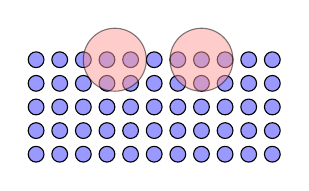
\begin{tikzpicture}
            % several particles
            % 4 row, 5 column
            \foreach \x in {0,1,2,3,4,5,6,7,8,9,10}
            \foreach \y in {0,1,2,3,4}
            \filldraw[fill=blue!40!white, draw=black] (0.3*\x,0.3*\y) circle (0.1);
            % draw a circle at the top row in the middle, alpha = 0.5
            \draw[fill=red!40!white, draw=black, opacity=0.5] (1.0,1.2) circle (0.4);
            % draw a circle at the top row in the middle, alpha = 0.5
            \draw[fill=red!40!white, draw=black, opacity=0.5] (2.1,1.2) circle (0.4);
        \end{tikzpicture}
    \end{figure}
    \begin{equation}
        \hat{\rho}_i = \frac{
            \sum_j m_j W_{ij}
        }{
            \sum_j \frac{m_j}{\rho_j}W_{ij}
        }
    \end{equation}
    据 SPHysics 中介绍,该修正方法可以有效地减小自由表面附近的误差。
    该步骤无需每步迭代都进行,一般每 10 步进行一次即可。
    也有推荐值 30 步一次。
    并且该核函数修正法也可以用于其他物理量的修正。
\end{frame}

\subsection{邻域搜索}

\begin{frame}
    \frametitle{\subsecname}
    因为 Lagrange 描述法中,每个粒子的所在位置是随时间变化的,
    所以需要在每一步迭代中都对每个粒子的光滑核半径内的邻域(支撑域)进行搜索。
    正常的实现每步都是复杂度为 $O(N^2)$ 的算法。

    一个较为直接的优化方法是将空间划分为背景网格,
    将每个粒子所在的网格单元的周围 9 个(二维)或 27 个(三维)单元的粒子都加入到该粒子的邻域搜索中。
    这样可以将搜索复杂度降低到 $O(N\log N)$。

    \begin{figure}[H]
        \centering
        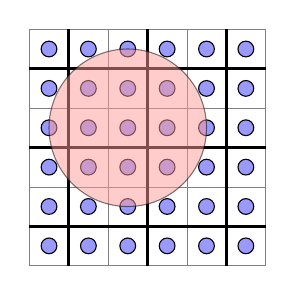
\begin{tikzpicture}
            % draw the background
            \draw[step=0.5cm,gray,very thin] (-1.5,-1.5) grid (1.5,1.5);
            % draw the main grid
            \draw[step=1cm,black,very thick] (-1.5,-1.5) grid (1.5,1.5);
            % draw the particles
            % random position
            \foreach \x in {-1.25,-0.75,...,1.25}
            \foreach \y in {-1.25,-0.75,...,1.25}
            \filldraw[fill=blue!40!white, draw=black] (\x,\y) circle (0.1);
            % draw the circle
            \draw[fill=red!40!white, draw=black, opacity=0.5] (-0.25,0.25) circle (1);
        \end{tikzpicture}
    \end{figure}
    这需要高级的数据结构的,
    自己手写的安全性和效率未必高。
    目前用了 MIT 协议的三方库,如果要自己实现需要 HashMap 和 KD-Tree。
\end{frame}

\subsection{固壁边界条件的实现}

\begin{frame}
    \frametitle{\subsecname}
    在查询了 SPHysics 的源代码以及一本河海大学老师写的书之后,
    我发现他们都采用了一种“虚拟粒子”的方法来实现固壁边界条件。
    \begin{figure}[H]
        \centering
        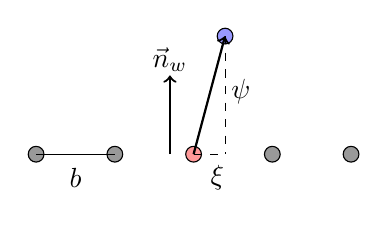
\begin{tikzpicture}
            \foreach \x in {0,1,3,4}
            \draw[fill=black!40!white, draw=black] (\x,0) circle (0.1);
            \draw[fill=blue!40!white, draw=black] (2.4,1.5) circle (0.1);
            \draw[fill=red!40!white, draw=black] (2,0) circle (0.1);
            
            \draw[->, thick] (2,0) -- (2.4,1.5);
            \draw[->, thick] (1.7,0) -- (1.7,1);
            \node at (1.7,1.2) {$\vec{n}_w$};
            \draw[dashed] (2.4,1.5) -- (2.4,0);
            \draw[dashed] (2, 0) -- (2.4,0);

            \draw[-] (0,0)--(1,0);
            \node at (0.5, -0.3) {$b$};

            \node at (2.6,0.8) {$\psi$};
            \node at (2.3, -0.3) {$\xi$};
        \end{tikzpicture}
    \end{figure}
    \begin{equation}
        \vec{f}_w=P(\psi)R(\xi)\epsilon(u_{\perp},z)\vec{n}_w
    \end{equation}
    $\psi$ 为粒子到壁面的距离,$\xi$ 为粒子到壁面粒子投影的距离,
    $u_{\perp}$ 为粒子在壁面法向的速度,$z$ 为粒子的水中深度,
    $\vec{n}_w$ 为壁面法向单位向量。
\end{frame}

\begin{frame}
    \frametitle{\subsecname}
    其中 $P(\xi)$ 计算公式如下:
    \begin{equation}
        P(\xi)=A\frac{1}{\sqrt{q}}(1-q)
    \end{equation}
    其中:
    \begin{equation}
        q=\frac{\psi}{2h}\quad A = 0.01\frac{1}{h}c_i^2
    \end{equation}
    事实上这里的壁面虚拟力的设置会发现极大,
    之前程序中 $\frac{1}{h}$ 忘了除发现可以正常算出来,
    但是除了以后发现程序反而容易炸(靠 bug 运行?)。
    $R(\xi)$ 的计算公式如下,是一个沿壁面周期性变化的函数:
    \begin{equation}
        R(\xi)=\frac{1}{2}\left[
            1+\cos\left(\frac{2\pi\xi}{b}\right)
        \right]
    \end{equation}
\end{frame}

\begin{frame}
    \frametitle{\subsecname}
    $\epsilon(u_{\perp},z)$ 的计算公式分为两部分:
    \begin{equation}
        \epsilon(u_{\perp},z)=\epsilon (u_{\perp})+\epsilon(z)
    \end{equation}
    其中:
    \begin{equation}
        \epsilon(u_{\perp})=
        \begin{cases}
            0 &\quad u_{\perp}\geq 0\\
            -\frac{20u_{\perp}}{c_0} &\quad -20u_{\perp}<c_0\\
            1 &\quad -20u_{\perp}\geq c_0
        \end{cases}
    \end{equation}
    \begin{equation}
        \epsilon(z)=
        \begin{cases}
            0 &\quad z\geq 0\\
            -\frac{z}{h_0} &\quad -h_0<z<0\\
            1 &\quad -h_0\geq z
        \end{cases}
    \end{equation}
    其中 $c_0$ 为声速,$h_0$ 为参考水深。
    这一项可以看出这两项是对粒子的移动速度和压力深度作了修正。
    靠近壁面速度大、压力深度大的粒子受到壁面的作用力也更大。
\end{frame}

\begin{frame}
    \frametitle{\subsecname}
    这里有一个问题,就在于这个壁面虚拟力的计算公式中,$A$ 这一项。
    我们考虑 $c_0=k\sqrt{gL}$,其中初始情况下,
    $L$ 为水的初始深度,$k$ 为一个常数一般取为 $10$。
    对于光滑核半径 $h$ 而言,总水深表示为 $L=nh$ 。
    这样的话,对于密度不大的情形,
    $A$ 这一项的数量级大约在:
    \begin{equation}
        A\sim 0.01\frac{1}{h}c_i^2\sim 0.01\frac{1}{h}k^2gL
        \sim 0.01\frac{1}{h}k^2gnh\sim 0.1k^2n
    \end{equation}
    这件事情就很奇怪,壁面力并不依赖于光滑核半径,
    而却依赖于水粒子的数量——也就是说为了匹配计算量级,
    用来离散计算域的粒子数量并不是越多越好,
    否则会导致壁面力过大。
    这边还需要再查和测试。
    \begin{figure}[H]
        \centering
        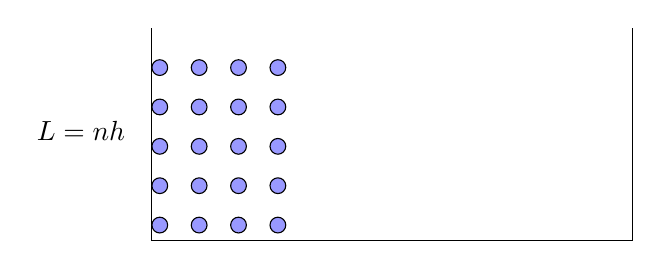
\begin{tikzpicture}
            \foreach \x in {0,1,2,3}
            \foreach \y in {0,1,2,3,4}
            \draw[fill=blue!40!white, draw=black] (0.5*\x,0.5*\y) circle (0.1);
            \draw[-] (-0.1,2.5)--(-0.1,-0.2)--(6,-0.2)--(6,2.5);
            \node at (-1,1.2) {$L=nh$};
        \end{tikzpicture}
    \end{figure}
\end{frame}

\subsection{CFL 数的文献支撑}

\begin{frame}
    \frametitle{\subsecname}
    经查询,CFL 数的计算公式与光滑核半径与人工声速有关,
    一般可以取为:
    \begin{equation}
        \Delta t = 0.1\frac{h}{c_0}
    \end{equation}
    当然上述公式的取法相当保守,
    为了加快计算速度,可以取为:
    \begin{equation}
        \Delta t = 0.1\frac{h}{V_{\max}}
    \end{equation}
    而人工声速至少是粒子速度的 10 倍,
    至此 $\Delta t,c_0,h,n_{\text{fluid}}$ 这几个参数已经耦合起来。
    当 $n_\text{fliuid}$ 较大(仿真分辨率提高)时,
    如前所述人工声速也会很大,
    这样边界力会异常大,产生数值不稳定。
    同时,如果缩小光滑核半径以缩小仿真的问题尺度,
    那么仿真时间步长也会变小,仿真时间会变长。
    这给我的程序 debug 造成了比较大的困扰。
\end{frame}

\subsection{多线程并行计算}

\begin{frame}
    \frametitle{\subsecname}
    为了提高程序的运行效率,我引入了多线程并行计算。
    这里先简单运用了线程锁的方式对程序进行了简单的并行计算。
    不过从计算效率来看,
    上锁的并行方式对并行效率是有影响的。
    对比与之前串行、未进行邻域搜索的 C++ 程序而言计算效率大概如下表所示:
    \begin{table}[H]
        \centering
        \begin{tabular}{c|c|c}
            \hline
            1800粒子 & $h/dr=1.5$ & $h/dr=3$ \\
            \hline
            C++ & 8it/s & 7it/s \\
            Julia+邻域搜索 & 30it/s & 21it/s \\
            Julia+邻域搜索+10线程 & 108it/s & 76it/s \\
            \hline
        \end{tabular}
    \end{table}
    当然我也在反思程序结构本身是不是不太适合并行,
    可能后面上 MPI 并行和 GPU 并行的时候需要先学一下并行原理,
    再对于程序结构进行重构。
\end{frame}

